\documentclass[10pt,a4paper]{book}
\usepackage[utf8x]{inputenc}
\usepackage{ucs}
\usepackage{amsmath}
\usepackage{amsfonts}
\usepackage{texments}
\usepackage{color}
\usepackage{xcolor}
\usepackage{graphicx}
\usepackage{listings}
\usepackage{tikz}
\makeatletter
\def\ScaleIfNeeded{%
\ifdim\Gin@nat@width>\linewidth
\linewidth
\else
\Gin@nat@width
\fi
}
\makeatother
\usepackage[bookmarksnumbered=true,bookmarksopen=true]{hyperref}
\author{Christian Brandt & Florian Thomas}
\title{Entwicklung webbasierter Software}
\date{Wintersemester 2011/2012}
\begin{document}
\begin{titlepage}
\begin{center}
\begin{figure}[htbp]
\centering

\includegraphics[width=8cm]{Pictures/THM_Logo.png}%
\end{figure}
\large{Fachbereich MNI - Mathematik, Naturwissenschaften \& Informatik}
\linebreak 
\linebreak
\linebreak
\linebreak
\linebreak
\linebreak
\linebreak
\LARGE{Entwicklung webbasierter Software}
\linebreak
\linebreak
\linebreak
\linebreak
\linebreak
\linebreak
\linebreak
\large{Prüfer}
\linebreak
\large{Martin Karry, MSc.}
\linebreak
\linebreak
\large{Prüflinge}
\linebreak
\large{Christian Brandt \& Florian Thomas}
\linebreak
\linebreak
\linebreak
\linebreak
\Large{Projekt: Treebook}
\linebreak
\normalsize{Ein soziales Netzwerk mit Anbindung an Facebook und flickr}
\linebreak
\linebreak
\normalsize{Wintersemester 2011/2012}
\begin{figure}[htbp]
\centering

\includegraphics[width=6cm]{Pictures/treebook_treelogo.png}%
\end{figure}
\linebreak
\linebreak
\linebreak
\linebreak
\end{center}
\end{titlepage}
\setcounter{page}{1}
\subsubsection{Eidesstattliche Erklärung}

\tableofcontents
\renewcommand{\chaptername}{}
\renewcommand{\thechapter}{}
\renewcommand{\thesection}{\arabic{section}}
\renewcommand{\thefigure}{\arabic{figure}}

\chapter{Einleitung}
Im Rahmen der Veranstaltung "Entwicklung webbasierter Software", geleitet von Herrn MSc. Martin Karry, soll zum Bestehen eine webbasierte Software entwickelt werden.
\chapter{Einführung}
Die hier beschriebene Software ist ein soziales Netzwerk, vergleichbar mit Facebook\footnote{\href{http://facebook.com/}{http://facebook.com/}
} oder Google+\footnote{\href{http://plus.google.com/}{http://plus.google.com/}}. Der Name "Treebook" leitet sich aus der Struktur der 
Freundschaften innerhalb dieser Software her. Dieses System ist angelehnt an das Circle-System von Google+\footnote{\href{http://www.youtube.
com/watch?v=BeMZP-oyOII}{http://www.youtube.com/watch?v=BeMZP-oyOII}}: Der Benutzer besitzt mehrere "Trees" in denen wiederum 
mehrere Benutzer enthalten sein können.

Treebook benutzt mehrere Application programming interfaces (nachfolgend kurz API) um die Funktionsmöglichkeiten der Software zu erweitern. 
Dem Benutzer ist es so mit Hilfe der API von Facebook möglich, sich mit seinen Facebook-Zugangsdaten bei Treebook anzumelden. Die API des 
Bilderdienstes Flickr\footnote{\href{http://flickr.com}{http://flickr.com}} wird verwendet um dem Anwender zu ermöglichen innerhalb von 
Treebook mit seinen auf Flickr bereitgestellten Fotos zu interagieren (Fotos ansehen, kommentieren, hochladen).

Der Anwender hat mehrere für ein soziales Netzwerk typische Aktionen zur Auswahl. Er kann Nachrichten (sogenannte "Posts") schreiben, die er 
mit von ihm ausgewählten "Trees" teilt. Leser einer Nachricht können diese kommentieren, mögen und im Gegensatz zu den bekannten sozialen 
Netzwerken auch Ablehnung zeigen.

Dem Benutzer steht ein eigenes Profil zur Verfügung, in dem er Informationen über sich, für die anderen Benutzer, veröffentlichen kann. Diese 
Informationen, sowie eventuelle Fotos können über die Privatsphäreneinstellung entweder mit allen angemeldeten Benutzern geteilt werden oder 
nur mit den eigenen Trees.

Eine Onlineversion von Treebook ist unter \textbf{http://treebook.florianthomas.net} verfügbar.
\chapter{Analyse}
Software, die in diesem Markt bereits existiert beinhaltet etablierte Namen wie Facebook, Twitter oder Google+. Diese haben eine Reichweite und Bekanntheit mit der es ein neues Produkt unmöglich aufnehmen kann. Deshalb wird in Treebook versucht gute Konzept aus diesen Branchengrößen zu extrahieren, eigene Ideen hinzuzufügen oder ihre APIs zu nutzen.

Standardmäßig ist es der Nutzer gewohnt in einem sozialen Netzwerk eigene Posts verfassen zu können, die von den Freunden im Netzwerk gelesen und kommentiert werden können. Im Gegensatz zu Twitter gibt es in Treebook kein Zeichenlimit für einen Post, da diese Begrenzung in Twitter auf Grund der maximalen Länge einer SMS eingeführt wurde\footnote{\href{http://www.quora.com/Twitter-Inc-company/What-is-the-rationale-behind-Twitters-15-character-limit-for-usernames}{http://www.quora.com/Twitter-Inc-company/What-is-the-rationale-behind-Twitters-15-character-limit-for-usernames}}, es in Treebook aber ohnehin nicht möglich ist Posts per SMS abzusetzen.
Um sich von anderen Marken abzusetzen ist es in der hier dokumentierten Software möglich neben einer Zustimmung("Liken" auf Facebook, +1 auf Google+) auch Ablehnung durch eine "Dislike"-Funktion zu äußern.

Bei den Privatsphäre-Einstellungen distanziert sich Treebook ganz bewusst von einer schwer zugänglichen und unverständlichen Struktur der Einstellungen wie etwa auf Facebook. Es gibt nur zwei mögliche Einstellungen, die der Nutzer vornehmen kann: "Für alle Nutzer auf Treebook sichtbar" oder "Nur für Nutzer in meinen Trees sichtbar". Diese Möglichkeiten beziehen sich auf Flickr-Fotos sowie auf den "Über mich" Bereich.

Die etablierten Freundschaftssysteme in den gängigen sozialen Netzwerken sind sehr verschieden:
\begin{list}{$\bullet$}{}
\item \textbf{Facebook :} direktes Freundschaftssystem mit möglichen Freundschaftslisten, aber schwer den Überblick zu behalten
\item \textbf{Google+ :} Follower-Prinzip, verschiedene Gruppen möglich ("Circles"), einfach zu bedienen
\item \textbf{Twitter :} Follower-Prinzip, Freunde können in Listen eingeteilt werden, aber kein Zwang dies zu tun
\end{list}
Nach Evaluierung der diversen Möglichkeiten entschieden sich die Entwickler von Treebook das \textbf{Freundschaftssystem von Google+} zu adaptieren.

Um möglichst viele Nutzer begeistern zu können sich bei Treebook anzumelden entschlossen ist ein Login per Facebook möglich ohne sich bei einem zusätzlichen Dienst registrieren zu müssen. Über 800 Millionen\footnote{\href{http://newsroom.fb.com/content/default.aspx?NewsAreaId=22}{http://newsroom.fb.com/content/default.aspx?NewsAreaId=22}} möglichen Benutzern kann so der Einstieg erleichtert werden. Ein normales Registrierungsformular wird dennoch angeboten um niemanden auszuschließen.

Bei der Auswahl eines geeigneten Foto-Hosters geht es zunächst um die Frage, ob man die Bilder selbst hosten möchte oder auf die API eines anderen Anbieters zugreifen. Die Treebook-Verantwortlichen entschieden sich für letzteres, da diese Möglichkeit angenehmer für Nutzer sowie Entwickler scheint. Die zwei Dienste, die hier in der engeren Auswahl waren, sind Flickr und Google Picasa\footnote{\href{http://picasa.google.com/}{http://picasa.google.com/}}. Ausgewählt wurde hier schließlich Flickr, da Picasa stark mit Google+ verwurzelt ist und die oAuth-Möglichkeiten bei Flickr besser sind.  
\section{Ruby on Rails}
Die Wahl der Programmiersprache für das Backend fiel auf \textbf{Ruby}\footnote{\href{http://www.ruby-lang.org/en/}{http://www.ruby-lang.org/en/}} mit dem dazugehörigen Web-Framework \textbf{Rails}\footnote{\href{http://rubyonrails.org/}{http://rubyonrails.org/}}. Diese Entscheidung hatte mehrere Gründe:
\lstset{language=bash}
\begin{list}{$\bullet$}{}
\item Da im Frontend Daten dynamisch per AJAX nachgeladen werden sollten, ist es sinnvoll zwischen Frontend und Server per JSON zu kommunizieren. Variablen in JSON-Objekte umzuwandeln geht in Ruby on Rails sehr einfach:
\begin{lstlisting}
@user = User.first
respond_to do |format|
  format.json { render json: @user }
end

# Ergebnis etwa: [{"name":"Mustermann","firstname":"Max","id":1}]
\end{lstlisting}
\item Es gibt viele gute Erweiterungen, zum Beispiel für die Benutzerauthentifizierung oder "Wrapper" um fremde APIs zu nutzen
\item Object-relation mapping (ORM)\footnote{\href{http://ar.rubyonrails.org/}{http://ar.rubyonrails.org/}} in Rails macht das Entwickeln schneller
\end{list}

\section{jQuery}
Der meiste für Treebook entwickelte JavaScript-Code basiert auf der JavaScript-Bibliothek \textbf{jQuery}\footnote{\href{http://jquery.com}{http://jquery.com}}. Mit jQuery hat es der JavaScript-Entwickler äußerst bequem, da er sich nicht mehr um Browser-Weichen\footnote{Browser-Weichen sind in JavaScript übliche Code-Verzweigungen, die die verfügbaren Informationen des Browsers auswerten, um möglichst viele Browser-Eigenheiten bei der Ausführung des Codes abzudecken. Dadurch soll erreich werden, dass dieselbe JavaScript-Anwendung in möglichst vielen Browsern funktioniert.} kümmern muss und die Code-Menge um ein Vielfaches schrumpft. Damit bleibt JavaScript-Code überschaubarer und leichter wartbar.

Ein Beispiel:\footnote{In den Code-Beispielen wird der Zugriff auf die jQuery-Bibliothek mit der Variablen \textit{jQuery} gekennzeichnet. Im Produktiveinsatz wird meistens \textit{\$} verwendet, um den Code noch schlanker zu halten.}

\begin{lstlisting}
jQuery(function() {
  // HTML-Element mit ID "message" einblenden
  // nachdem die Seite fertig geladen ist
  jQuery('#message').fadeIn();
});
\end{lstlisting}

Desweiteren verfügt jQuery über eine auf CSS3 basierende Selector-Engine, die es dem Entwickler ermöglicht schnell an gewünschte DOM-Elemente\footnote{Document Object Model bezeichnet den baumartigen Aufbau einer auf XML basierenden Struktur.} zu gelangen und diese zu manipulieren.

jQuery stellt viele Funktionen bereit, die DOM-Tree-Manipulationen erheblich vereinfachen. Mehr dazu ist in der offiziellen jQuery-API\footnote{\href{http://api.jquery.com}{http://api.jquery.com}} nachzulesen.

\chapter{Installation}
Stellen Sie zunächst sicher, dass eine Internetverbindung besteht und die Ports \textbf{3000} und \textbf{9292} nicht durch andere Anwendungen belegt sind.
\section{Linux}
\begin{enumerate}
\item Laden Sie die aktuelle Ruby-Version (Stand 6.4.2012) von der offiziellen Ruby-Website herunter\footnote{\href{http://ftp.ruby-lang.org/pub/ruby/1.9/ruby-1.9.3-p125.tar.gz}{http://ftp.ruby-lang.org/pub/ruby/1.9/ruby-1.9.3-p125.tar.gz}} entpacken und installieren es wie jedes andere Programm unter Linux (evtl. werden dazu Root-Rechte benötigt).
\lstset{language=bash}
\begin{lstlisting}
# ./configure
# make
# make install
\end{lstlisting}
\item Führen Sie folgenden Befehl in der Konsole aus (eventuell mit Root-Rechten)
\begin{lstlisting}
# gem install bundler
\end{lstlisting}
Anschließen laden Sie bitte Ihre Shell neu.
\item Sie benötigen eine JavaScript Runtime auf dem Zielsystem. Falls noch keine vorhanden ist, wird Node.js\footnote{\href{http://nodejs.org/}{http://nodejs.org/}} empfohlen.
\item Kopieren Sie den Ordner \textbf{treebook.tar.gz} von der mitgelieferten DVD an einen beliebigen Ort innerhalb Ihres Home-Verzeichnisses und führen Sie anschließend folgende Befehle in der Konsole aus:
\begin{lstlisting}
# cd /pfad/zum/treebook/verzeichnis
# tar -zxvf treebook.tar.gz
# cd treebook
# bundle install
# rake db:migrate
\end{lstlisting}
\item \textbf{Optional:} Führen Sie
\begin{lstlisting}
# rake db:seed
\end{lstlisting}
aus, um Beispieldaten (Benutzer, Trees und Posts) zu laden.
\item Geben Sie
\begin{lstlisting}
# foreman start
\end{lstlisting}
in Ihrer Konsole ein um den Server zu starten und öffnen Sie anschließend die URL \textbf{http://localhost:3000} in Ihrem Browser.
\end{enumerate}
\section{Windows}
\begin{enumerate}
\item Laden Sie sich zunächst die aktuelle Version des \textbf{Rails Installers}\footnote{\href{http://railsinstaller.org/}{http://railsinstaller.org/}} herunter und folgen Sie den Installationsanweisungen.
\item Entpacken Sie den Ordner \textbf{treebook.tar.gz} von der mitgelieferten DVD in einen beliebigen Ort innerhalb Ihres Home-Verzeichnisses, öffnen sie anschließend eine Eingabeaufforderung im \textbf{Treebook}-Ordner und geben Sie folgende Befehle ein:
\begin{lstlisting}
# bundle install
# rake db:migrate
\end{lstlisting}
\item \textbf{Optional:} Führen Sie
\begin{lstlisting}
# rake db:seed
\end{lstlisting}
aus, um Beispieldaten (Benutzer, Trees und Posts) zu laden.
\item Geben Sie
\begin{lstlisting}
# foreman start
\end{lstlisting}
in Ihrer Konsole ein um den Server zu starten und öffnen Sie anschließend die URL \textbf{http://localhost:3000} in Ihrem Browser.
\end{enumerate}
\chapter{Backend}
\lstset{language=Ruby}
\section{Allgemeines}
Das Grundgerüst des Backends von Treebook besteht aus \textbf{Ruby on Rails}\footnote{\href{http://rubyonrails.org/}{http://rubyonrails.org/}}
, dem mitgelieferten Webserver \textbf{WEBrick}\footnote{\href{http://en.wikipedia.org/wiki/WEBrick}{http://en.wikipedia.org/wiki/WEBrick}}, 
dem Nachrichtenserver \textbf{Faye}\footnote{\href{http://faye.jcoglan.com/}{http://faye.jcoglan.com/}}, sowie einer \textbf{SQLite3}\footnote{\href{http://www.sqlite.org/}{http://www.sqlite.org/}} gestützten Datenbank.

\subsection{Datenbank}
Das Schema der Datenbank von Treebook:
\begin{figure}[htbp]
\centering
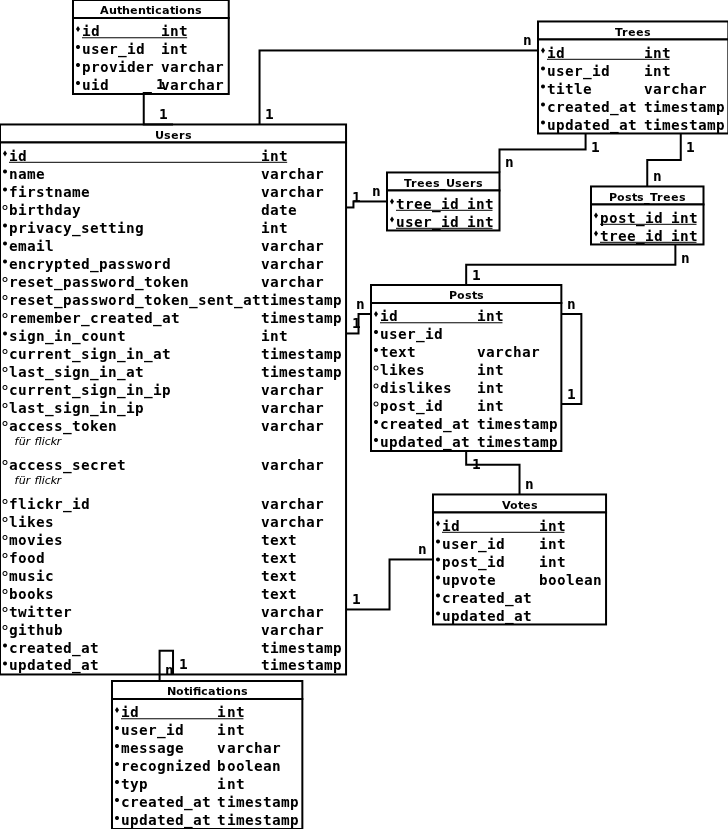
\includegraphics[width=\ScaleIfNeeded]{Pictures/db.png}%
\caption{Datenbankschema}%
\end{figure}

\subsection{Actions}
Die in den einzelnen Controllern definierten Methoden werden als \textbf{Actions} bezeichnet, da Sie nicht dazu verwendet werden, von anderem Code aufgerufen zu werden, sondern durch HTTP-Requests im Frontend (GET, POST, PUT oder DELETE). Dabei wird in den Actions jeweils ein JSON-Objekt zurückgegeben, welches im Frontend weiter verarbeitet werden kann.
Beispiel \textbf{show}-Action im \textbf{TreesController}
\begin{lstlisting}
# Gibt den Tree zurueck, oder falls
# dieser nicht dem aktuellen User gehoert, eine Fehlermeldung
def show
  @tree = Tree.find(params[:id])

  respond_to do |format|
    if @tree.user == current_user
      format.json { render json: @tree.to_json(:include => { :user => 
      	{:only => [:firstname, :name, :id, :email]}, :users => 
      	{:only => [:firstname, :name, :id, :email], :methods => :image}}) }
    else
      format.json { render json: "Du kannst leider nicht auf diesen Tree zugreifen", 
      	status: :unprocessable_entity }
    end
  end
end
\end{lstlisting}
\subsection{Routing}
In der Datei \textbf{/config/routes.rb} werden die Routen definiert, die als HTTP-Request abgesetzt werden müssen, um auf eine bestimmte Action zuzugreifen.
Beispiel:
\begin{lstlisting}
match "comment/" => "users#comment", :via => :post
\end{lstlisting}
\textbf{Bedeutet:} Ein HTTP POST-Request auf "http://localhost:3000/comment/" wird auf die Action \textbf{comment} im \textbf{UsersController} gemapt.
\section{Gems}
Als Gems (deutsch: Edelsteine) werden in Ruby Erweiterungen bezeichnet, die der Entwickler zu seiner Software hinzufügen kann. Folgende Gems werden in Treebook verwendet:
\subsection{Devise}
Devise wird zur Benutzerauthentifizierung verwendet. Es hilft dabei, Benutzern den Zugriff auf Funktionen des Controllers zu erlauben bzw. zu verbieten. Desweiteren ermöglicht es den Zugriff auf die Daten des momentan eingeloggten Anwenders.
\subsection{Omniauth-Facebook}
Erweiterung von Devise um per \textbf{OAuth}\footnote{\href{http://oauth.net/}{http://oauth.net/}} einen Login mit Facebook zu ermöglichen. 
Dafür wurde zunächst eine Treebook-App auf Facebook erstellt, der der Anwender bei erstmaligem Klick auf "Via Facebook anmelden" Zugriff auf 
die grundlegenden Daten seines Facebook-Accounts gewähren muss. In Treebook wurde im \textbf{OmniauthCallbacksController} eine Funktion 
definiert, die die von Facebook übermittelten Daten übergeben bekommt und anhand dieser entscheidet, ob ein neuer Benutzer angelegt werden muss oder ein bestehender Benutzer eingeloggt wird.
\subsection{Omniauth-Flickr}
Funktionsweise wie oben, allerdings wird hier nicht der Login per Flickr ermöglicht, sondern nur der Zugriff auf die Fotos des Treebook-Nutzers. Dazu wird der Benutzer bei der erstmaligen Verbindung gebeten, der Trebook-App die nötigen Rechte einzuräumen:
\begin{figure}[htbp]
\centering
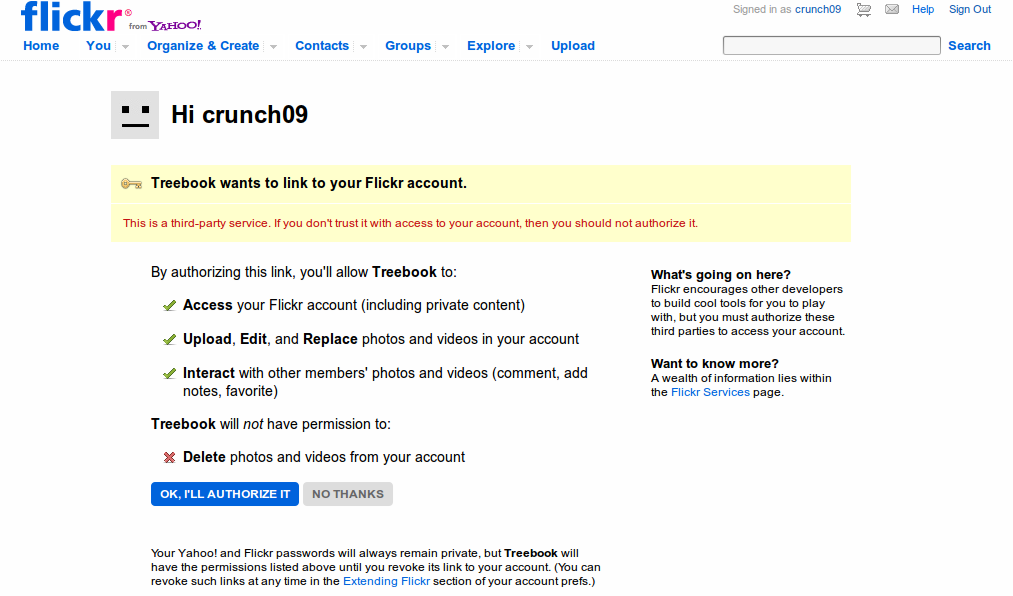
\includegraphics[width=\ScaleIfNeeded]{Pictures/screen_flickr_auth.png}%
\caption{Flickr Authentifizierung}%
\end{figure}
Die \textbf{flickrcallback}-Action im \textbf{UsersController} nimmt den Callback von Flickr entgegegen und speichert das übergebene Token in der Datenbank.
\subsection{Flickraw}
Das Flickraw-Gem\footnote{\href{https://github.com/hanklords/flickraw}{https://github.com/hanklords/flickraw}} ist eine Funktionsbibliothek, 
die den Zugriff auf die Flickr-API erleichtert. Initialisiert wird es mit dem \textbf{API-Key} und \textbf{Shared-Secret} der Trebook-App auf Flickr.
\begin{lstlisting}
FlickRaw.api_key = "XYZ"
FlickRaw.shared_secret = "020b6b5209"
\end{lstlisting}
In der Users-Tabelle der Datenbank sind drei Attribute für die Flickr-Authentifizierung des Benutzers wichtig: \textbf{flickr\_id} , 
\textbf{access\_token} und \textbf{access\_secret}. Die letzten beiden werden speziell für Request mit Schreibrechten benötigt. Eine Funktion im User-Model ist deshalb speziell dafür gedacht zu überprüfen, ob der Benutzer eine Flickr-Verbindung eingerichtet hat
\begin{lstlisting}
def got_flickr_connection?
  !self.access_token.nil? && !self.access_secret.nil?
end
\end{lstlisting}
Hier als Beispiel die \textbf{upload\_photo} Action, welche die von \textbf{Devise} bereitgestellte Variable \textbf{current\_user} benutzt,
um auf den aktuell eingeloggten Nutzer zuzugreifen und Parameter aus dem Frontend empfängt. Näheres dazu im Abschnitt \textbf{Routing}.
\begin{lstlisting}
def upload_photo
  flickr = FlickRaw::Flickr.new

  if current_user.got_flickr_connection?
    flickr.access_token = current_user.access_token
    flickr.access_secret = current_user.access_secret
    @response = flickr.upload_photo params[:photo].tempfile.path, 
    				:title => params[:title], 
    				:description => params[:description]
  else
    @response = "Du hast leider noch keine Flickr-Verbindung hergestellt"
  end

  respond_to do |format|
    format.json { render json: @response }
  end
end
\end{lstlisting}
\subsection{Faye}
Faye ist ein \textbf("publish-subscribe" Nachrichtensystem), welches außerdem einen extra Server für diesen Zweck bereitstellt. So können alle Nutzer, die die benötigten Rechte besitzen in Echtzeit informiert werden, wenn ein neuer Post verfasst wurde. Dazu muss im Backend nur eine von Faye bereitgestellte JavaScript-Datei zusaetzlich geladen werden. Der Code, der im Frontend implementiert werden muss, wird spaeter in dieser Dokumentation noch genauer erlaeutert.
\subsection{Gon}
Gon hilft dabei, die Kommunikation zwischen Backend und Frontend zu vereinfachen. So wird im Backend eine Variable \textbf{gon.user\_id} mit der Id des aktuell angemeldeten Benutzers belegt.
\begin{lstlisting}
gon.user_id = current_user.id
\end{lstlisting}
Diese Variable steht nun im Frontend zur Verfügung und kann im Javascript-Code ausgelesen werden.
\subsection{Foreman}
Foreman ermöglicht es mehrere Server mit einem Befehl zu starten(in Treebook sind das WEBrick und Faye). Die zu startenden Server werden in \textbf{/Procfile} definiert.
\section{Sonstiges}
\subsection{Gravatar}
Gravatar\footnote{\href{http://gravatar.com}{http://gravatar.com}} ist ein Dienst, der es ermöglicht zu einer Email-Adresse ein Avatar zu hinterlegen. Treebook nutzt diesen Dienst für die Darstellung der Nutzer-Avatare. Der Vorteil dieser Lösung liegt für den Anwender darin, dass er seinen gewünschten Avatar an einer zentralen Stelle verwalten kann und nicht direkt in Treebook hochladen muss. Gravatar stellt eine API bereit, die es ermöglicht aus der Email-Adresse des Treebook-Nutzers die Gravatar Bild-URL zu berechnen, sowie einene Fallback-Avatar anzugeben.
\begin{lstlisting}
def image
  default_url = "http://localhost:3000/assets/derp.png" # Default-Bild
  gravatar_id = Digest::MD5.hexdigest(self.email.downcase)
  img = "http://gravatar.com/avatar/#{gravatar_id}.png?s=40" +
        "&d=#{CGI.escape(default_url)}"
  img # die letzte Anweisung im Code einer Methode wird zurueckgegeben
end
\end{lstlisting}
\chapter{Frontend}
\section{Allgemeiner Aufbau}
Die Anwendung wird generell in mehreren Schritten geladen. Serverseitig wird zunächst das HTML-Grundgerüst zur Verfügung gestellt, in das nach und nach die gewünschten Inhalte geladen werden.
Dies ermöglichen verschiedene JavaScript-Funktionen, welche neue Informationen per "Asynchronous JavaScript and XML" (kurz AJAX) vom Server abrufen.
Wann und welche Informationen genau vom Server bereitgestellt werden, wird in den folgenden Abschnitten erläutert.

\section{Der Anwendungsstart}
Im Allgemeinen wird beim ersten Besuch der Treebook-Seite die Startseite mit dem Treebook-Logo angezeigt.
\begin{figure}[htbp]
\centering
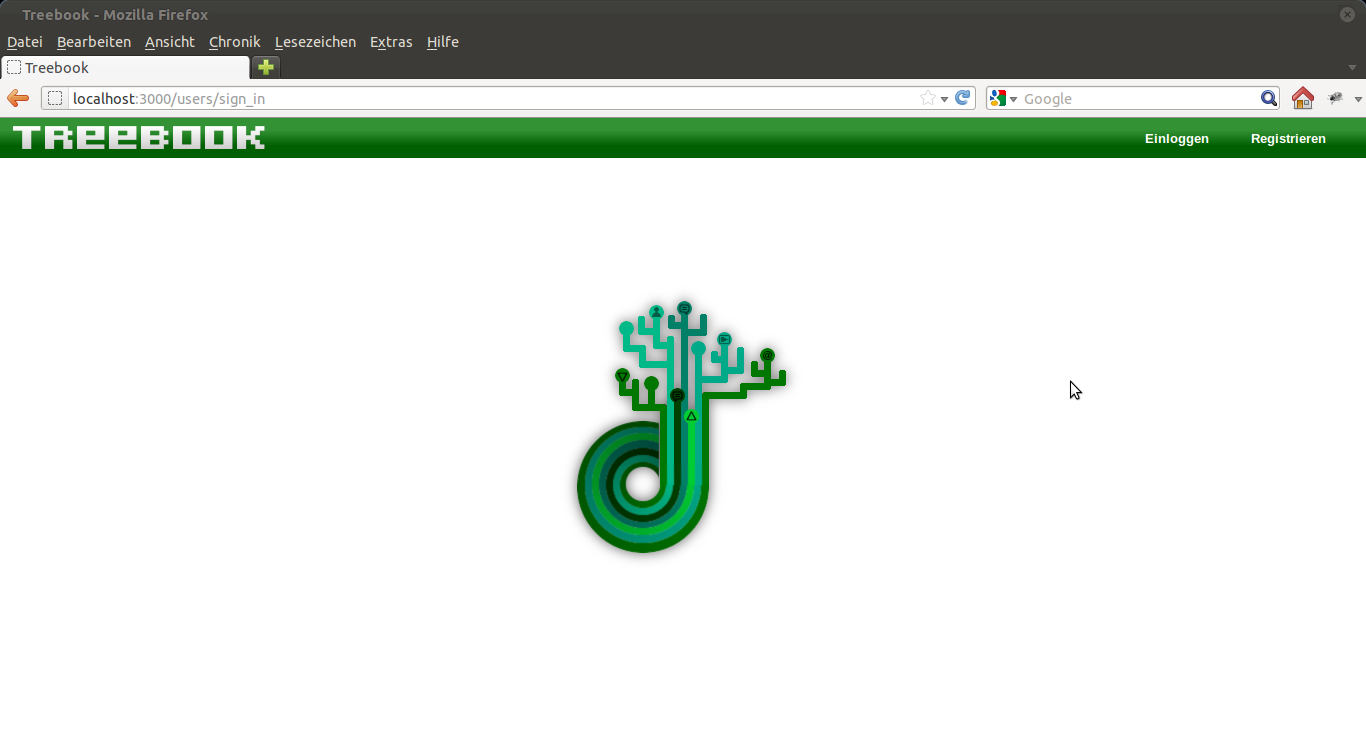
\includegraphics[width=\ScaleIfNeeded]{Pictures/screen_startup.png}%
\caption{Startseite}%
\end{figure}
Von hier aus hat der Anwender die Möglichkeit sich im System anzumelden oder zu registrieren.
Die Anmeldung erfolgt wahlweise über eine dem System bekannte E-Mail-Adresse und dem dazugehörigen Passwort oder über die Facebook-OAuth-API ("Via Facebook anmelden").
Ist der Nutzer dem System noch nicht bekannt, kann er sich dennoch direkt via Facebook anmelden. In diesem Fall wird für ihn ein neues Treebook-Nutzerkonto mit seinen bei Facebook hinterlegten Daten angelegt.

\section{Nach dem Login}
\subsection{Der Stream}
Nachdem sich der Anwender angemeldet hat, sieht er zunächst den sogenannten \textbf{Stream} vor sich. Links davon befindet sich die allgemeine \textbf{Navigation} mit seinen erstellten Trees. Rechts befindet sich ein Suchfeld.
\begin{figure}[htbp]
\centering
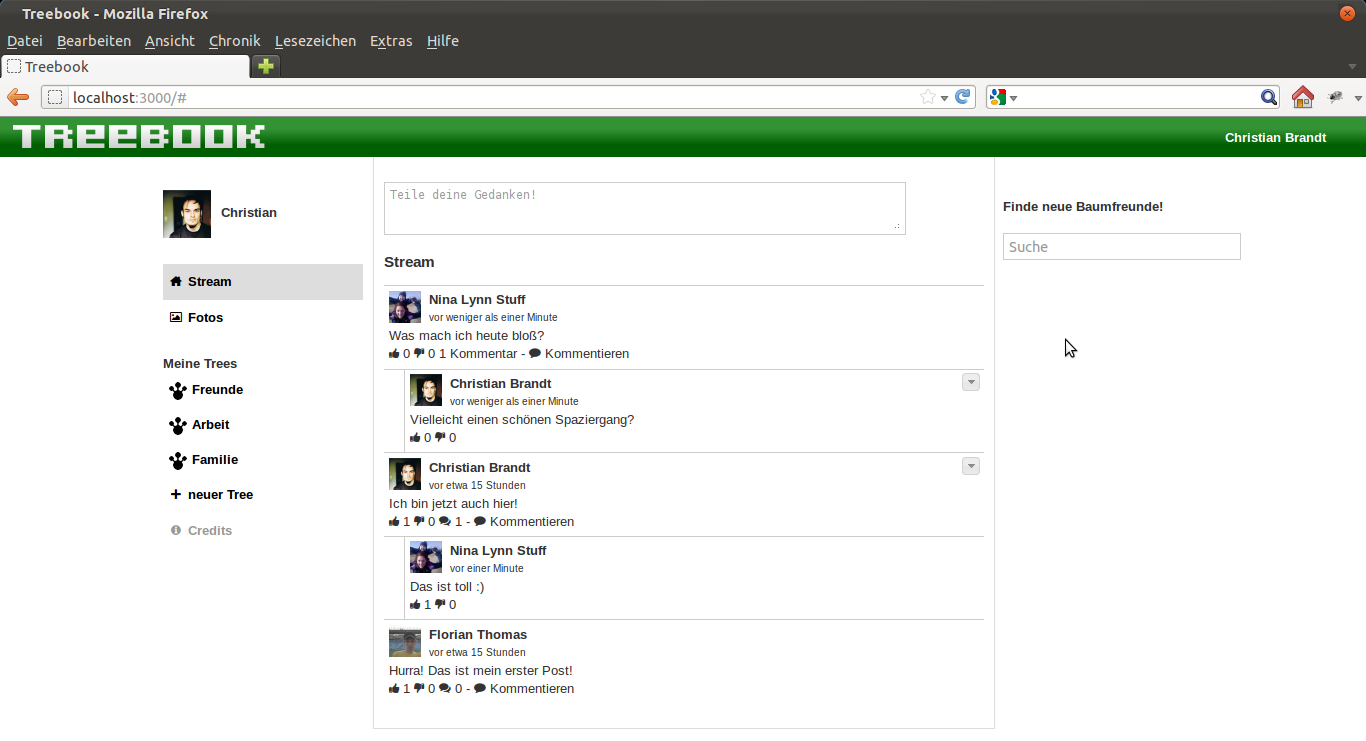
\includegraphics[width=\ScaleIfNeeded]{Pictures/screen_stream.png}%
\caption{Stream}%
\end{figure}
Im Stream werden alle \textbf{Posts} angezeigt, die der Anwender selbst, oder Kontakte in seinen Trees erfasst haben. Diese sind rückwärts sortiert nach Erstellungsdatum, sodass der Anwender am Seitenanfang immer die neuesten Posts sieht und, je weiter er nach unten scrollt, die Posts immer älter werden.
Unter jedem Post werden (sofern vorhanden) die letzten 3 \textbf{Kommentare} zu diesem Post angezeigt. Sind mehr als 3 Kommentare verfügbar, sieht der Anwender einen Link "Alle vorherigen Kommentare anzeigen", welcher nach einem Klick die übrigen Kommentare zum Post anzeigt.
\subsection{Die Navigation}
Die Navigation teilt sich in 4 Unterbereiche auf:
\begin{list}{$\bullet$}{}
\item Das \textbf{Profilbild} und der Vorname des derzeit eingeloggten Nutzers
\item Allgemeine Links zum Stream und zu den \textbf{Fotos} des eingeloggten Nutzers
\item Die vom Nutzer erstellten Trees und ein Link zum Erstellen eines neuen Trees
\item Ein Link zu den \textbf{Credits}
\end{list}
Per Klick auf das Profilbild oder den Vornamen des Anwenders wird das Profil geladen. Standardmäßig sieht der Anwender dann seine eigenen Beiträge aufgelistet.

Mit einem Klick auf "Fotos" wird ebenfalls das Profil des Nutzers geladen, allerdings wird direkt der Foto-Reiter aktiviert.

Klickt der Nutzer auf einen \textbf{Tree}, so werden nur Beiträge angezeigt, die diesem Tree zugeordnet sind, also Beiträge, die vom User explizit für diesen Tree freigegeben wurden, oder Beiträge von Kontakten, die der Nutzer diesem Tree zugeordnet hat.

Ein Klick auf "neuer Tree" zeigt ein Textfeld, in das der Nutzer eine Bezeichnung für den Tree eingibt und zwei Buttons zum Speichern oder Verwerfen des neuen Trees.

Hinter den \textbf{Credits} verbergen sich Links zu Software und sonstigen Ressourcen, die für die Entwicklung von Treebook verwendet wurden.

\subsection{Die Tree-Ansicht}
Klickt der Nutzer auf einen Tree in der Navigation, so befindet sich der Stream in der \textbf{Tree-Ansicht}. Hier werden nur Posts angezeigt, die diesem Tree zuzuordnen sind. Das sind Posts, die der Nutzer diese Tree freigegeben hat, oder Posts von Kontakten, die der Nutzer diesem Tree zugeordnet hat.
\begin{figure}[htbp]
\centering
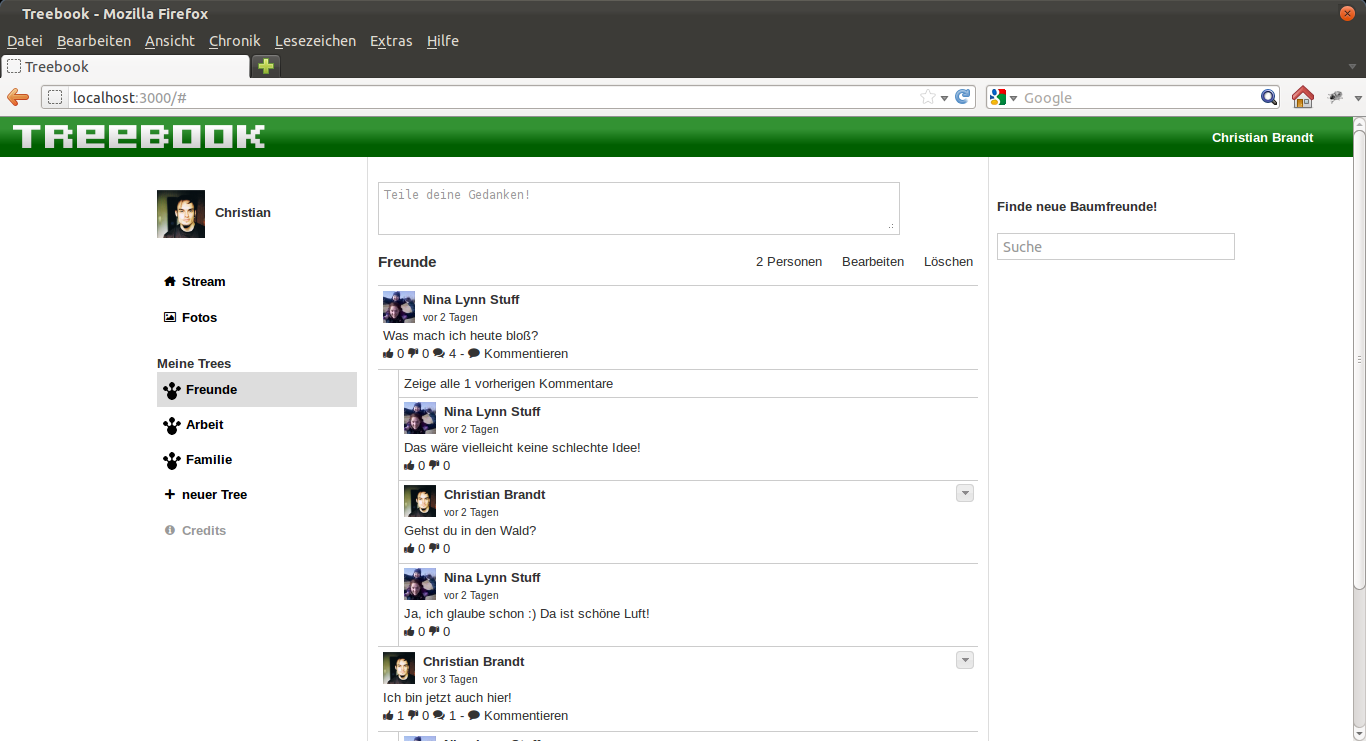
\includegraphics[width=\ScaleIfNeeded]{Pictures/screen_treeview.png}%
\caption{Tree-Ansicht}%
\end{figure}
In der Tree-Ansicht befinden sich rechts neben dem Titel 3 Aktionsbuttons:
\begin{list}{$\bullet$}{}
\item \textbf{Die Anzahl der Personen in diesem Tree}

Zeigt nach einem Klick eine Liste aller Personen, die diesem Tree zugeordnet wurden.
\item \textbf{Bearbeiten}

Bietet dem Nutzer die Möglichkeit, den Tree umzubenennen.
\item \textbf{Löschen}

Löscht den Tree inklusive der Kontaktzuordnungen zu diesem Tree.
\end{list}

\subsection{Das Suchfeld}
Das Suchfeld zur Rechten des Streams bietet dem Anwender die Möglichkeit nach Personen zu suchen. Nachdem er mindestens 3 Buchstaben eingetippt hat, liefert das System alle Personen, deren Vor- oder Nachname mit diesen Buchstaben beginnt. Eine Suche nach "Han" wird genauso "Hans Dampf" wie "Lars Hansen" liefern, sofern diese Personen bei Treebook registriert sind.
\begin{figure}[htbp]
\centering
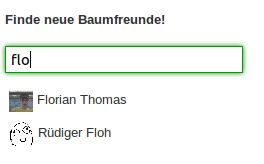
\includegraphics[width=\ScaleIfNeeded]{Pictures/screen_search.png}%
\caption{Suche}%
\end{figure}
Der Anwender hat nun die Möglichkeit per Klick auf einen Namen das Profil des jeweiligen Nutzers aufzurufen, welches dann im mittleren Bereich der Seite angezeigt wird.
Er hat weiterhin die Möglichkeit den Namen per \textbf{Drag and Drop} auf einen Tree in der linken Navigation zu ziehen. Dies fügt den Nutzer dann in den ausgewählten Tree ein, sofern er nicht bereits dem Tree zugeordnet wurde.

\subsection{Der Stream}
Im Stream werden alle Posts und deren Kommentare angezeigt, die vom Nutzer selbst oder seinen Kontakten verfasst wurden. Die Posts sind nach Datum sortiert, wobei die neuesten weiter oben stehen.
Ein Post beinhaltet im Allgemeinen folgende Inhalte:
\begin{list}{$\bullet$}{}
\item Das Profilbild und den vollen Namen des Autors, sowie der ungefähre Zeitraum, der seit dem Veröffentlichen des Posts vergangen ist
\item Den Text, den der Autor verfasst hat
\item Die Anzahl der \textbf{Likes} ("positive Bewertungen"), \textbf{Dislikes} ("negative Bewertungen") und \textbf{Kommentare} zu diesem Post
\item Einen Link zum \textbf{Kommentieren} dieses Posts
\end{list}
\begin{figure}[htbp]
\centering
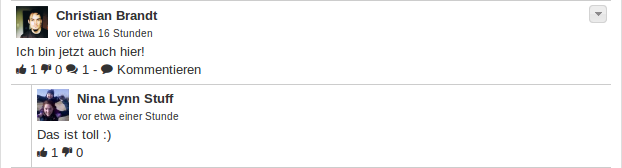
\includegraphics[width=\ScaleIfNeeded]{Pictures/screen_post.png}%
\caption{Post}%
\end{figure}
Sofern der Autor des Posts der aktuelle Nutzer ist, wird in der oberen rechten Ecke des Posts ein kleiner Button mit einem nach unten weisendem Pfeil angezeigt. Bei Klick auf diesen Button öffnet sich ein kleines Kontext-Menü zum \textbf{bearbeiten} und \textbf{löschen} des Posts. Bei erneutem Klick auf den Button wird das Kontext-Menü wieder ausgeblendet.
\begin{figure}[htbp]
\centering
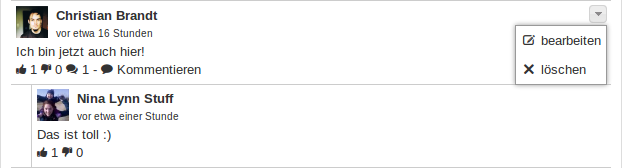
\includegraphics[width=\ScaleIfNeeded]{Pictures/screen_post_menu.png}%
\caption{Post mit Kontext-Menü}%
\end{figure}
Unterhalb des Posts werden die Kommentare eingerückt angezeigt. Diese sind im Wesentlichen genauso aufgebaut, wie ein Post. Allerdings können Kommentare nicht ebenfalls kommentiert werden, daher entfällt die Anzahl der Kommentare und der Link zum Kommentieren.
Standardmäßig werden die bis zu letzten 3 Kommentare zu einem Post angezeigt. Wurde ein Post mehr als dreimal kommentiert, so erscheint zwischen Post und den letzten 3 Kommentaren ein Link "Zeige alle x vorherigen Kommentare", der nachdem er geklickt wurde alle vorherigen Kommentare anzeigt.
\begin{figure}[htbp]
\centering
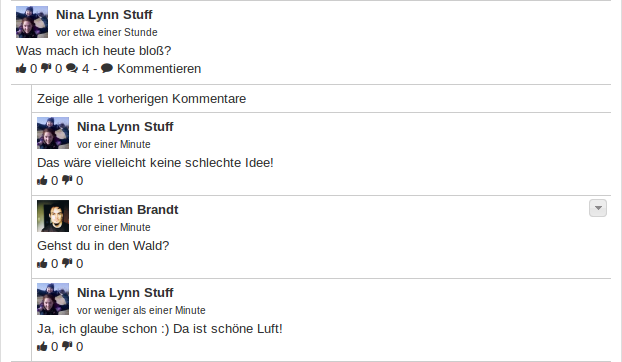
\includegraphics[width=\ScaleIfNeeded]{Pictures/screen_post_and_comments.png}%
\caption{Post mit mehr als 3 Kommentaren}%
\end{figure}
Auch ein Kommentar kann bearbeitet und gelöscht werden, wenn der Nutzer diesen verfasst hat. Dies geschieht analog zur Bearbeitung eines Posts.

\subsection{Die Kopfzeile}
In der Kopfzeile wird zu jeder Zeit der Treebook-Schriftzug angezeigt, der den Link zur Startseite enthält. Am rechten Rand sieht der Nutzer nochmals seinen vollen Namen, hinter dem sich ein Link zu seinem Profil und zum Ausloggen verbirgt.
Nach dem Ausloggen landet der Nutzer wieder auf der Startseite mit dem Treebook-Logo.

Links neben seinem Namen, sieht der Nutzer einen Indikator für Benachrichtigungen. Hier wird angezeigt, wieviele Benachrichtigungen für den aktuellen nutzer vorliegen. In folgenden Fällen wird eine Benachrichtigung generiert:
\begin{list}{$\bullet$}{}
\item wenn ein anderer Nutzer einen Post des Anwenders kommentiert hat
\item wenn ein anderer Nutzer ein Foto des Anwenders kommentiert hat
\item wenn ein anderer Nutzer den Anwender in einen seiner Trees aufgenommen hat
\end{list}
Mit einem Klick auf den Indikator werden die Benachrichtigungen angezeigt. Danach werden diese vom System als gelesen markiert und beim nächsten Aufruf der Liste nicht mehr angezeigt.
\subsection{Das Profil}
Das Profil eines jeden Nutzers gliedert sich in 3 Bereiche auf:
\begin{list}{$\bullet$}{}
\item Den Kopfbereich, der das Profilbild und den vollen Namen des Nutzers anzeigt
\item Die Profil-Navigation, mit der man zwischen den Beiträgen, den persönlichen Informationen und den Fotos des Nutzers hin- und herschalten kann
\item Die Inhaltsanzeige, die je nach ausgewähltem Pofil-Navigationselement, den entsprechenden nhalt anzeigt
\end{list}

Das Profilbild wird über \textbf{Gravatar}\footnote{\href{http://gravatar.com}{http://gravatar.com}} verwaltet. Betrachtet der Anwender sein eigenes Profil, so erscheint beim Überfahren des Profilsbilds mit der Maus ein kleiner Button zum Bearbeiten des Profilbildes. Dieses verlinkt nach Gravatar, wo der Anwender sein Profilbild ändern kann.

Unter \textbf{Beiträge} sind alle für den Anwender zugänglichen Posts des Nutzers aufgelistet. Posts, die der Anwender nicht sehen soll, wird er auch hier nicht sehen.

Ein Klick auf \textbf{Über mich} zeigt alle persönlichen Profilinformationen des Nutzers, sofern der Anwender sie sehen darf. Besucht der Anwender seine eigene "Über Mich"-Seite, so kann er einerseits seine Privatsphären-Einstellung, andererseits seine persönlichen Profilinformationen bearbeiten.
Bei Treebook stehen folgende persönliche Informationen zur Bearbeitung zur Verfügung:
\begin{list}{$\bullet$}{}
\item Ich mag
\item Filme
\item Essen
\item Musik
\item Bücher
\item Twitter
\item Github
\end{list}
Die Privatsphären-Einstellung legt fest, welche Treebook-Nutzer seine persönlichen Informationen und seine Fotos sehen dürfen.

Klickt der Anwender auf \textbf{Fotos}, wird er einen der folgenden Inhalte sehen:
\begin{list}{$\bullet$}{}
\item Die Fotos des Nutzers, sofern der Anwender sie sehen darf
\item Einen Hinweis, dass der Nutzer noch keine Fotos erstellt hat
\end{list}
oder, sofern der Anwender ein eigenes Profil aufruft:
\begin{list}{$\bullet$}{}
\item Seine Fotos
\item Einen Hinweis, dass der Anwender jetzt seinen Treebook-Account mit seinem flickr-Konto verknüpfen kann
\end{list}
Wenn Fotos vorhanden sind, werden zunächst nur die Alben des Nutzers als \textbf{Thumbnails} angezeigt. Beim Überfahren mit der Maus erscheinen die bis zu 4 ersten Fotos dieses Albums in einer Miniatur-Ansicht.
Nach Klick auf ein Album werden die enthaltenen Fotos als Thumbnails dargestellt. Zusätzlich wird, wenn das Fotoalbum den Anwender gehört, ein "Plus"-Icon angezeigt, hinter dem sich ein Foto-Upload-Dialog verbirgt.
Nach einem Klick auf ein Foto wird dieses in der Großansicht geöffnet.
In der Großansicht werden außerdem die Kommentare zu diesem Foto sowie ein Formular zum Kommentieren angezeigt. Gehört das Foto dem Anwender, so kann er dessen Titel und Beschreibung bearbeiten.
\section{Verwendete Techniken}
\subsection{jQuery-UI}
\textbf{jQuery-UI}\footnote{\href{http://jqueryui.com}{http://jqueryui.com}} ist eine Erweiterung für jQuery, die eine erweitere Effekt-Auswahl, sowie eine beliebig anpassbare und steuerbare Oberflächen-Gestaltung von einigen HTML-Elementen bietet.
Mit jQuery-UI lässt sich ein einheitliches Aussehen auf HTML-Seiten erreichen, ohne dafür viel Aufwand betreiben zu müssen. jQuery-UI legt Wert auf Benutzerfreundlichkeit, die Einhaltung von Webstandards, Barrierefreiheit und flexibles Styling.

\subsection{AJAX}
Dank der in jQuery integrierten Unterstützung für AJAX-Abfragen, kann die Treebook-Anwendung auf dieser Technologie aufbauend die Kommunikation mit dem Rails-Server durchführen.
Überwiegend findet der Datenabruf im \textbf{JSON}\footnote{JavaScript Object Notation}-Format statt. Die jQuery-interne ajax-Methode lässt sich durch den \textit{dataType}-Parameter leicht steuern, sodass der Inhalt der abgerufenen Seite automatisch interpretiert wird. Im Falle von JSON ist der Rückgabewert kein String, sondern bereits ein fertiges JavaScript-Objekt.

Ein Beispiel für eine GET-Anfrage um den Post mit der ID 1 abzurufen:
\begin{lstlisting}
jQuery.ajax({
  url: 'posts/1.json',
  type: 'GET',
  dataType: 'json',
  success: function(postObject) {
    // postObject beinhaltet die JSON-Antwort
    console.log(postObject);
  }
});
\end{lstlisting}

Der Vorteil von AJAX liegt vorallem darin, dass die Menge an übertragenen Daten gering gehalten wird, da nicht die komplette Seite mit jedem Aufruf eines Links neu ausgeliefert wird, sondern lediglich die Informationen, die gerade benötigt werden.
Bei Treebok sind dies in den meisten Fällen JSON-Objekte, die dann direkt verwertet werden können.

\subsection{Faye}
Die Erweiterung von Treebook durch \textbf{Faye} ermöglicht es, dass alle Benutzer immer automatisch die neuesten Posts und Kommentare sehen.
Jeder Benutzer hat seinen eigenen \textbf{Channel} (deutsch: Kanal). Wenn der Benutzer einen neuen Post oder Kommentar abschickt, wird die neue ID des Posts bzw. Kommentars über seinen Channel übertragen.
Zeitgleich hat jeder Benutzer einen registrierten Listener auf alle Channels seiner verknüpften Kontakte. Sobald eine Nachricht auf einen der Channels registriert wird, prüft das System, ob der neue Post bzw. Kommentar für den aktuellen Nutzer relevant ist. Ist dies der Fall, so wird der Post bzw. Kommentar direkt angezeigt.

Um den Lesefluss nicht zu beeinträchtigen, werden neue Posts und Kommentare nur direkt angezeigt, wenn sie sich unterhalb der aktuellen Ansicht des Nutzers befinden.
Neuere Posts werden zwar an den Anfang des Streams gehängt, jedoch nicht direkt angezeigt, da sonst möglicherweise die Seite permanent nach unten "hüpfen" würde.
Stattdessen wird einfach ein Link am Anfang des Streams eingeblendet, der den Nutzer darüber informiert, wieviele neue Posts gerade registriert worden sind. Erst nach einem Klick auf diesen Link werden alle neuen Posts und Kommentare eingeblendet.

\subsection{Font Awesome}
Zur Ergänzung der Benutzerführung verwendet Treebook das Icon-Set von \textbf{Font Awesome}\footnote{\href{http://fortawesome.github.com/Font-Awesome/}{http://fortawesome.github.com/Font-Awesome/}}.
Die Icons von Font Awesome lassen sich sehr einfach in HTML-Seiten einbinden und sind voll skalierbar, da sie als Vektorgrafiken hinterlegt sind.
Der Einbau eines solchen Icons kann an jeder beliebigen Stelle im HTML-Dokument erfolgen.
\begin{figure}[htbp]
\centering
\begin{lstlisting}
<li>
  <a href="#" name="addTree" onclick="addTree()">
    <i class="icon-plus"></i> neuer Tree
  </a>
</li>
\end{lstlisting}
\caption{Einbindung eines Font Awesome-Icons}%
\end{figure}
Dies fällt kürzer aus, als die Einbindung über ein \textit{img}-Tag und ist bequemer zu handhaben, da sich die Icons an der Schriftgröße orientieren und somit optimal ausgerichtet sind. \textit{img}-Tags müssen in der Regel per CSS noch extra ausgerichtet werden.

\chapter{Fazit}

\chapter{Literatur}
\begin{list}{$\bullet$}{}
\item Facebook-API für Webseiten

https://developers.facebook.com/docs/guides/web/
\item fancybox

http://fancybox.net
\item flickr-API

http://www.flickr.com/services/api/
\item Font Awesome

http://fortawesome.github.com/Font-Awesome
\item jQuery

http://jquery.com
\item jQuery-UI

http://jqueryui.com
\item Ruby on Rails

http://rubyonrails.org
\end{list}
\end{document}